\section{Les technologies du Big Data:}
Cette technologie est importante pour présenter une analyse plus précise qui conduit l’analyste d’affaires à prendre des décisions très précises, assurant ainsi une efficacité opérationnelle plus considérable en réduisant les coûts et les risques commerciaux. Maintenant, pour implémenter de telles analyses et détenir une telle variété de données, il faut avoir besoin d’une infrastructure qui puisse faciliter et gérer et traiter d’énormes volumes de données en temps réel. De cette façon, le Big Data est classé en deux sous-catégories, le Big Data opérationnel qui comprend des données sur des systèmes et le Big Data analytique qui comprend des systèmes. 

Nous décrivons ensuite ici tous les composants qui font partie des solutions Big Data sous de nombreux angles : matériel, méthodologies, logiciels et applications de base, etc.

Pour mieux catégoriser ces concepts, nous les avons a répartis en différentes sections selon l'objectif visé par chacun. Ces catégories sont : l'infrastructure, le stockage, le traitement et les composants de haut niveau.

\subsection{Les infrastructures :}
Le développement du Big Data commence avec les clusters Big Data qui exécutent en parallèle les instructions d'un logiciel de haut niveau. Le cluster est artitionné en deux types de nœuds selon la fonction principale exercée:

\begin{itemize}[label=\textbullet]
	\item Nœuds de données ou esclaves (informatique).
	\item Nœuds de gestion ou maîtres (gestion).
\end{itemize}

Outre leur fonction, le maître et les esclaves peuvent être différenciés par leurs capacités de calcul et leur quantité dans le champ de nœuds.

Les esclaves sont chargés de surveiller les données partitionnées, de traiter et d'interroger les données locales. Les unités de données et de traitement doivent être aussi proches que possible pour éviter les retards introduits par les mouvements entre les partitions. Les nœuds de données sont gourmands en disque et standard en termes de capacités de calcul et de mémoire.

Les maîtres reçoivent et transforment les programmes des applications clientes en instructions parallèles qui peuvent être comprises par les esclaves. Une fois que les applications clientes ont atteint le démon maître, elles finissent par démarrer ou réveiller plusieurs processus dans les esclaves qui retournent finalement une sortie suivant la direction opposée. Parmi l'ensemble des responsabilités approuvées pour les nœuds de gestion figurent :

\begin{itemize}[label=\textbullet]
	\item La récupération après défaillance.
	\item La gestion des ressources.
	\item La planification des travaux.
	\item La surveillance ou la sécurité.
\end{itemize}

Pour accomplir ces tâches, les maîtres nécessitent une puissance de calcul et de mémoire élevée. Dans les clusters Big Data standard, il suffit de garder deux maîtres supports qui se surveillent mutuellement.

Les deux types de nœuds sont connectés via une connexion réseau, généralement LAN (Ethernet ou InfiniBand). Certaines configurations permettent également de connecter les maîtres de déférents centres de données sur un réseau WAN pour éviter facilement les défaillances du système. Dans chaque centre de données, le maître et les esclaves sont interconnectés en privé pour ingérer des données, déplacer des données entre les nœuds et effectuer des requêtes. Il existe également un autre réseau public qui sert de façade entre le client et le service de gestion (SSH, VNC, interface web,..)

\subsection{Les technologies de traitements :}

\begin{figure}[h]
	\centering
	
\includegraphics[scale=0.4]{img/part1/1.8}
	\caption{Hadoop.}
\end{figure}

Dans cette section nous parlerons de l'arrivée des technologies de traitement ajustées, plus spécialement sur la mise au point de modes de calcul à haute performance ( MapReduce ), nous parlerons de ( Hadoop ) une solution de Big Data très largement utilisée pour effectuer des analyses sur de très grands nombres de données.

\begin{enumerate}[label=\protect\ding{\value*}, start=182,font=\color{blue}]
\item \subsubsection{Map-reduce :}
MapReduce a été introduit par Google et décrit en détails dans la publication « MapReduce : Simplified Data Processing on Large Clusters » publiée en 2004 et ça pour faciliter la mise en œuvre de ses workfows de traitement parallèle. L'objectif principal était de remplacer la programmation complexe et non intuitive sur l'informatique distribuée (préalablement abordée par les plateformes HPC) par une plateforme transparente moderne avec seulement deux fonctions : Map et Reduce. Ces deux fonctions définies par l'utilisateur permettent aux utilisateurs d'utiliser les ressources distribuées sans se plaindre du réseau, de la planification, de la récupération après défaillance, etc.

Un modèle aussi intuitif que le MapReduce ne nécessite pas d'expertise concernant le parallélisme et les systèmes distribués. Son Framework Plug-and-Play embarque tous les détails pour implémenter les systèmes de calcul parallèle, la persistance et la résilience, l'optimisation et l'équilibre des ressources.

\begin{itemize}[label=\ding{51}]
\item \textbf{Principe de MapReduce :}
MapReduce applique le principe dit « diviser pour distribuer pour régner », la stratégie mise en place pour exécuter un calcul sur des données massives consiste a : 
\begin{itemize}[label=\textbullet]
\item \textbf{Découper} les données en sous ensemble de plus petite taille, appelés lors ou fragments.
\item \textbf{Affecter} chaque lot a une machine permettant ainsi leur traitement en parallèle.
\item \textbf{Agréger} l'ensemble des résultats intermédiaires obtenu pour chaque lot pour construire le résultat final.
\end{itemize}
\newpage
Ce dernier se repose sur deux fonctions : Map qui permet aux différents points du cluster distribué de distribuer leur travail. La fonction Reduce qui permet de réduire la forme finale des résultats des clusters en un seul résultat.

Le rôle du développeur d’applications distribuées c’est de réfléchir en MapReduce :
\begin{itemize}[label=\textbullet]
\item Choisir une manière de découper les données afin que l’opération MAP soit parallèlisable. 
\item Choisir la clé a utilisé pour le problème ciblé.
\item Ecrire le code de la fonction pour l’opération MAP.
\item Ecrire le code de la fonction pour l’opération REDUCE.

\end{itemize}
\subparagraph{Exemple d'utilisation de MapReduce:}
\textit{Nous allons tester un programme MapReduce grâce à un exemple très simple, le WordCount, l'équivalent du HelloWorld pour les applications de traitement de données. Le Wordcount permet de calculer le nombre de mots dans un fichier donné, en décomposant le calcul en deux étapes:
L'étape de Mapping, qui permet de découper le texte en mots et de délivrer en sortie un flux textuel, où chaque ligne contient le mot trouvé, suivi de la valeur 1(pour dire que le mot a été trouvé une fois)
et l'étape de Reducing, qui permet de faire la somme des 1 pour chaque mot, pour trouver le nombre total d'occurrences de ce mot dans le texte.}

\begin{figure}[h]
	\centering
	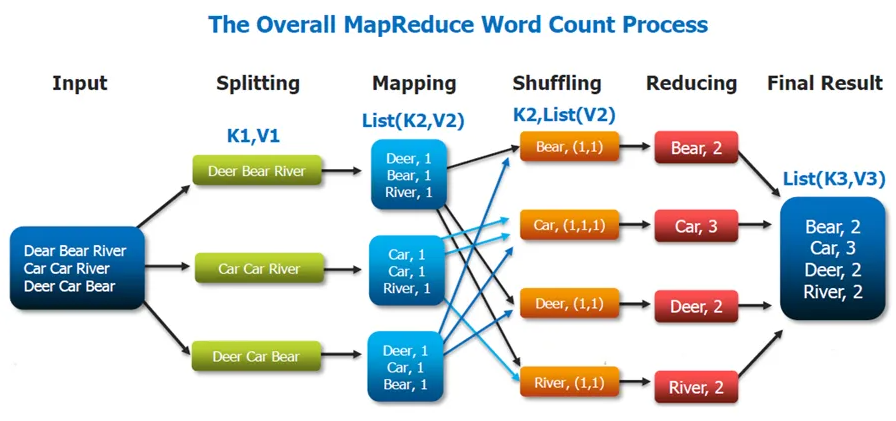
\includegraphics[scale=0.6]{img/part1/1.9}
	\caption{Exemple de Word Count.}
\end{figure}

\item \textbf{Les avantages de MapReduce: }Parmi les avantages de la programmation MapReduce nous citons
\begin{itemize}[label=\textbullet]
	\item La scalabilité.
	\item La flexibilité.
	\item La sécurité et l'authentification.
	\item Le traitement parallèle.
	\item La disponibilité.
	\item Un modèle simple de programmation.
\end{itemize}

\end{itemize}

\item \subsubsection{HADOOP:}
MapReduce a tout son intérêt dans le Big Data car il permet le passage à l’échelle des traitements sur de gros volumes de données, cependant il faut une infrastructure logiciel dédiée qui permettent d’exécuté le schéma MapReuce de manière distribué sur les clusters machine. C’est là qu’intervient Hadoop.

Hadoop est un framework logiciel open source permettant de stocker des données, et de lancer des applications sur des grappes (cluster) de machines standards. Cette solution offre un espace de stockage massif pour tous les types de données, une immense puissance de traitement et la possibilité de prendre en charge une quantité de tâches virtuellement illimitée. Basé sur Java, ce framework fait partie du projet Apache, sponsorisé par Apache Software Foundation.

Grâce a MapReduce, il permet de traiter les immenses quantités de données. Plutôt que de devoir déplacer les données vers un réseau pour procéder au traitement, MapReduce permet de déplacer directement le logiciel de traitement vers les données. 

Hadoop se compose essentiellement de :

\begin{figure}[h]
	\centering
	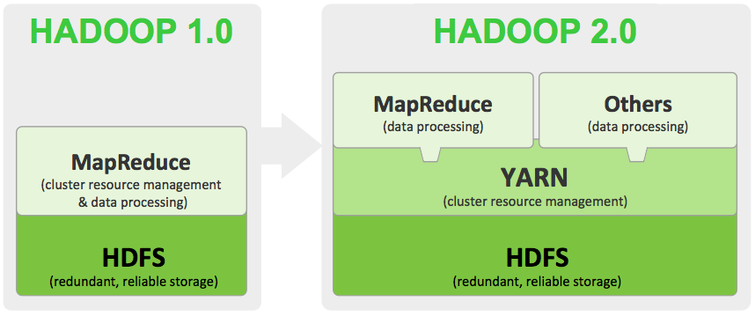
\includegraphics[scale=0.4]{img/part1/1.10}
	\caption{Les composants d'Hadoop.}
\end{figure}

\begin{itemize}[label=\ding{51}]
\item \textbf{Système de gestion de fichiers HDFS (Hadoop Distributed File System) :} HDFS est un système de fichiers distribué, extensible et portable Inspiré par GFS et écrit en Java. Il est conçu pour être un système de stockage distribué, évolutif et résilient, conçu pour interagir facilement avec MapReduce. Il fournit une bande passante d'agrégation importante tout au long du réseau. Comme pour GFS, un réseau HDFS est composé d'un nœud maître appelé Namenode et des serveurs de données appelés Datanodes, de grande taille par défaut 64 Mo pour optimiser les temps de transfert et d'accès. Il est toutefois possible de monter à 128 Mo, 256 Mo, 512 Mo voire 1 Go.
\item \textbf{Modèle de programmation Map-reduce :} Le framework MapReduce permet de traiter les immenses quantités de données. Plutôt que de devoir déplacer les données vers un réseau pour procéder au traitement, MapReduce permet de déplacer directement le logiciel de traitement vers les données. Ce modèle fera l'objet de la deuxième technologie que nous allons présenter.
\item \textbf{YARN (Yet Another Ressource Negiciator)}à été ajoutée comme une fonctionnalité clé depuis Hadoop 2.0 déployée en 2013, Avant son ajout, Hadoop ne pouvait exécuter que des applications MapReduce. YARN a donc beaucoup augmenté les cas d’usage potentiels du framework. En découplant la gestion des ressources et la planification du composant de traitement de données de MapReduce, YARN a également permis à Hadoop de prendre en charge davantage d’applications et de types de traitement différents.

\end{itemize}

Hadoop 3 sortie le 13 décembre 2017 apporte son lot de nouveautés qu’il convient de présenter:
\begin{itemize}[label=\textbullet]
\item La première différence provient de la gestion des conteneurs. La troisième apporte davantage d’agilité grâce à l’isolation des paquets de Docker.
\item Le coût d’utilisation d’Hadoop 3 est également plus faible. La deuxième version demande plus d’espace de stockage. Là où la troisième version demande 9 blocs de  stockage.
\item Autre différence majeure, Hadoop 2 ne gère qu’un seul namenode. Cet outil de gestion de l’arborescence du système de fichiers, les métadonnées des fichiers et les répertoires. La version suivante peut en gérer plusieurs, ce qui permet d’augmenter de manière exponentielle la taille des infrastructures.
\item Enfin, cette dernière version du système HDFS ouvre de nouvelles perspectives pour les concepteurs d’algorithmes de machine learning et de deep learning. 
\end{itemize}

\item \subsubsection{Les bases de données NoSQL :}
De nos jours, l'ubiquité de la connexion Internet est une réalité (les voitures que nous conduisons, les montres que nous portons, nos petits appareils médicaux domestiques, nos réfrigérateurs et congélateurs, nos Smartphones et ordinateurs portables). De plus, les données numériques produites par les êtres humains, dont les séquences vidéo, les photos et autres, atteignent des volumes importants de plusieurs EO par jour. Ces données actuellement stockées dans des bases qui leur ont été conçues spécifiquement sont gérés par des logiciels de gestion de bases de données volumineuses, jouant le rôle d'intermédiaires entre les bases de données d'un côté et les applicatifs et leurs utilisateurs de l'autre. On parle ici des bases de données non-relationnelles, dites NoSQL. 

Concrètement une base de données NoSQL est une approche de la conception des bases et de leur administration particulièrement utile pour de très grands ensembles de données distribuées. Elle englobe une gamme étendue de technologies et d'architectures, afin de résoudre les problèmes de performances en matière d'évolutivité et de Big Data que les bases de données relationnelles ne sont pas conçues pour affronter. De plus elle est particulièrement utile lorsqu'une entreprise doit accéder, à des fins d'analyse, à de grandes quantités de données non structurées ou de données stockées à distance sur plusieurs serveurs virtuels du Cloud.

\begin{figure}[h]
	\centering
	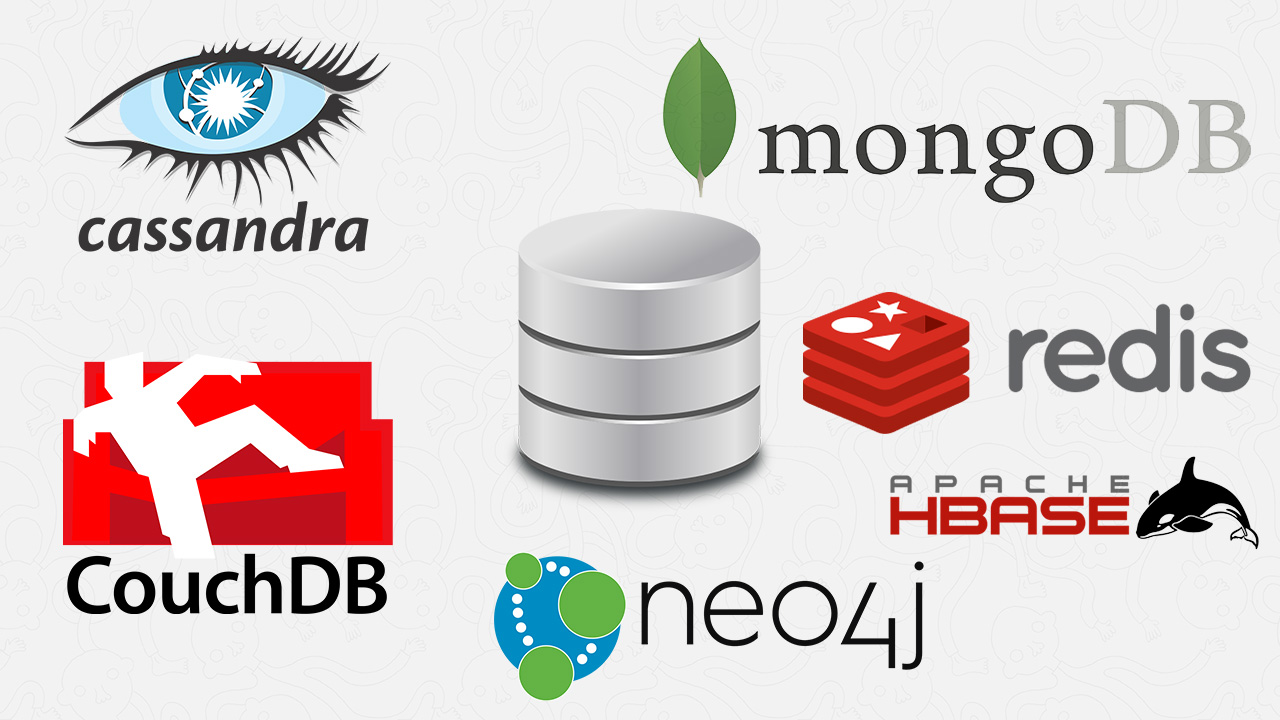
\includegraphics[scale=0.2]{img/part1/1.11}
	\caption{Bases de données NoSql.}
\end{figure}

\end{enumerate}

\subsection{Les technologies de stockage :}
\begin{enumerate}
\item  \textbf{Stockage "In-Memory" :}
Pour des analyses encore plus rapides, les traitements directement en mémoire sont une solution. Une technologie bien qu'encore trop coûteuse il est vrai pour être généralisée. Les bases de données "In Memory" sont généralement construites comme des base relationnelles. Elles sont conformes aux exigences ACID (Atomicity, Consistency, Isolation, Durability) qui garantissent l'intégrité des transactions. Les données contenues en mémoire sont volatiles par principe. Un système de sauvegarde périodique par image disque, snapshot, permet de sauvegarder la base. Ce système est complété d'une historisation des transactions afin de remettre la base en état en cas de coupure de courant.

\item \textbf{Le Cloud computing :}
C’est une solution d'externalisation capable de louer de puissants moyens de calcul. Ceux-ci sont dotés de larges capacités de stockage extensibles et adaptés aux traitements des Big Data. Au cœur des réflexions sur les infrastructures IT, de nouvelles offres Big data as a Service (BDaaS).

C'est un terme général employé pour désigner la livraison de ressources et de services à la demande par Internet. Il désigne le stockage et l'accès aux données par l'intermédiaire d'Internet plutôt que via le disque dur d'un ordinateur. Il s'oppose ainsi à la notion de stockage local, consistant à entreposer des données ou à lancer des programmes depuis le disque dur.

\end{enumerate}

\cite{fernandez_les_2017}
